\documentclass[a4paper,12pt,french]{article}

\usepackage[cours]{../../Style}

%\selectcolormodel{cmyk}

%\usepackage{wrapfig}
%\makeatletter
%\setlength{\parskip}{1ex}
%\newcommand{\@minipagerestore}{\setlength{\parskip}{1ex}}

% Début du document
%%%%%%%%%%%%%%%%%%%
\begin{document}

\title{Variables aléatoires}
\maketitle

\begin{programme}
\item Variable aléatoire discrète: Loi de probabilité, espérance
\item Loi de Bernoulli $(0;1)$ de paramètre $p$, espérance
\item Capacités:
\begin{itemize}
\item Interpréter en situation les écritures $\{X=a\}$, $\{X \leq a \}$ et calculer les probabilités correspondantes $\Pro(X=a)$ et $\Pro(X \leq a)$
\item Calculer et interpréter en contexte l'espérance d'une variable aléatoire discrète
\item Reconnaitre une situation aléatoire modélisée par une loi de Bernoulli.
\item Simuler $N$ échantillons de taille $n$ d'une loi de Bernoulli et représenter les fréquences observées des 1 par un histogramme ou un nuage de points
\item Interpréter sur des exemples la distance à $p$ de la fréquence observée des 1 dans un échantillon de taille $n$ d'une loi de Bernoulli de paramètre $p$
\end{itemize}
\item Probabilité associée à une expérience aléatoire à deux épreuves indépendantes
\item Probabilité associée à une répétition d'épreuves aléatoires identiques et indépendante de Bernoulli
\item Capacités
\begin{itemize}
\item Représenter par un arbre de probabilités une expérience aléatoire à deux épreuves indépendantes et déterminer les probabilités des évènements associés aux différents chemins.
\item Représenter par un arbre de probabilités la répétition de $n$ épreuves aléatoires identiques et indépendantes de Bernoulli avec $n \leq 4$ afin de calculer des probabilités
\end{itemize}
\end{programme}

\begin{ex}
On lance pièce équilibrée. Si on tombe sur pile, on gagne 2\euro, sinon on perd 1\euro. On note $X$ les gains après un lancer. Ainsi $X$ peut valoir soit $2$, soit $-1$. La probabilité que $X$ vaille 2, notée $\Pro(X=2)$, vaut $\frac 1 2 = 0,5$.
\end{ex}

\begin{defin}

VAR = fonction $\Omega \rightarrow \R$

\end{defin}

\begin{ex}
\compo[0.58]
{
On reprend l'exemple ci-dessus, mais $X$ représente cette fois les gains après deux lancers successifs. On peut représenter les possibilités grâce à l'arbre ci-contre.

On a alors:
\begin{itemize}
\item  $\Pro(X=1)=\frac 2 4 = 0,5$;
\item $\Pro(X=-2)=\frac 1 4=0,25$.
\end{itemize}
}
{
\begin{center}
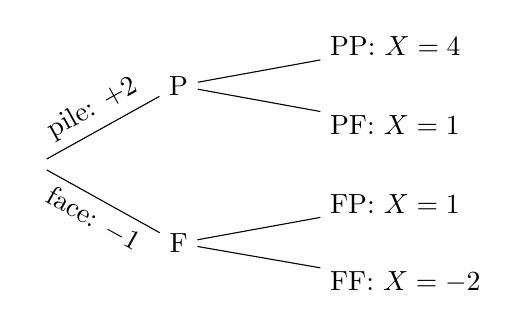
\begin{tikzpicture}[x=1.8cm] % Même effet que xscale=2 mais l'option sloped marche

\node (O) at (0,0) {};
\node (P) at (1,1) {P};
\node (F) at (1,-1) {F};
\node[anchor=west] (PP) at (2,1.5) {PP: $X=4$};
\node[anchor=west] (PF) at (2,0.5) {PF: $X=1$};
\node[anchor=west] (FP) at (2,-0.5) {FP: $X=1$};
\node[anchor=west] (FF) at (2,-1.5) {FF: $X=-2$};

\draw (O) -- (P) node[midway,above,sloped] {pile: $+2$} (P) -- (PP) (P) -- (PF) (O) -- (F) node[midway,below,sloped] {face: $-1$} (F) -- (FP) (F) -- (FF);
\end{tikzpicture}
\end{center}
}
\end{ex}

\section{Généralités}
\Def{Soit $\Omega:=\{ \omega_{1},\dots ,\omega_{n} \}$ un ensemble fini qu'on appelle univers. Les $(\omega_{i})$ sont appelés issues possibles.}
\begin{ex}
Pour un lancer de dé à 6 faces on prendra $\Omega=\{ 1,2,3,4,5,6\}$.

\end{ex}
Dans la suite fixons un univers $\Omega$.
\Def{Une \textbf{variable aléatoire} réelle notée $X$ est une fonction de $\Omega \longrightarrow \R$.}

Ainsi, une variable aléatoire c'est affecter à chaque issue possible une valeur.\\
\begin{center}
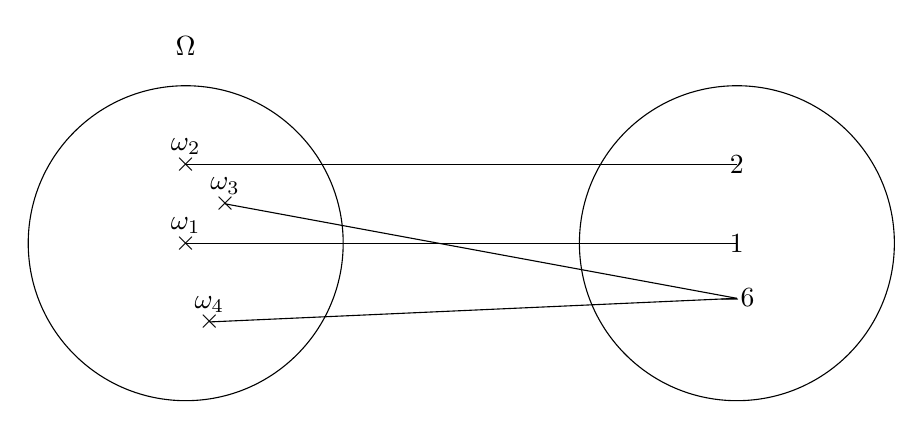
\begin{tikzpicture}
\draw (-2,-2) circle (2cm);
\draw (-2,-2) node{$\times$};
\draw (-2,-2) node[above]{$\omega_{1}$};
\draw (-2,-1) node{$\times$};
\draw (-2,-1) node[above]{$\omega_{2}$};
\draw (-1.5,-1.5) node{$\times$};
\draw (-1.5,-1.5) node[above]{$\omega_{3}$};
\draw (-1.7,-3) node[above]{$\omega_{4}$};
\draw (-1.7,-3) node{$\times$};
\draw (-2,0.5) node{$\Omega$};
\draw (5,-2) circle (2cm); 
\draw (5,-2) node{$1$};
\draw (5,-1) node{$2$};
\draw (5,-2.7) node{$-6$};
\draw (-2,-2)--(5,-2);
\draw (-2,-1)--(5,-1);
\draw (-1.5,-1.5)--(5,-2.7);
\draw (-1.7,-3)--(5,-2.7);
\end{tikzpicture}
\end{center}
\\\\
\underline{Notation:}\\
$\bullet $ L'événement "$X$ prend la valeur $a$" est notée $X=a$.\\ Par exemple, si on reprend la schéma ci-dessus l'évément $X=6$ est réalisé pour les issues $\omega_{3}$ et $\omega_{4}$.\\\\
$\bullet$ L'événement "$X$ inférieur ou égale à $a$" est notée $X\leq a$.\\
Par exemple ici, $X\leq 2$ est obtenue pour les issues $\omega_{2}$ et $\omega_{1}$.
\begin{ex}
On considère un dé à $6$ faces. On associe à chaque numéro des faces une valeur de gain potentielle.
\begin{align*}
    1\longrightarrow -2\euro{}\\
    2,3\longrightarrow -10\euro{}\\
    5\longrightarrow 50\euro{}\\
    4,6\longrightarrow -50\euro{}\\
\end{align*}
Ici, on associe aux issus possibles $\{ 1,2,3,4,5,6 \}$ un élément de l'ensemble $\{ -2,-10,50,-50\}$. On définit ainsi une variable aléatoire $X$.\\
\begin{enumerate}[leftmargin=2cm ]
\item L'événement "$X=-50$" est vérifié pour les issues $4,6$.
\item 
L'événement "$X\leq -10$" est vérifié pour les issues $2,3,1$.
\end{enumerate}
\end{ex}
\begin{de}
Si $X$ est à valeur dans $\{0,1\}$ on parle \textbf{d'épreuve de Bernouilli}.
\end{de}
\begin{ex}
On effectue une épreuve de pile ou face, on peut définir une variable aléatoire $X$ qui a l'événement pile associe 1 et à face 0. Cette variable aléatoire ainsi définie est une épreuve de Bernouilli.
\end{ex}
\section{ Loi de probabilité & Espérance}
\subsection{ Loi de probabilité}
\Def{ Soit $\Omega$ un univers et $X$ une VAR telle que pour tout $i$, $X=a_{i}$ avec $a_{i}\in \R$. \\
Définir la loi de probabilité de $X$, c'est associé à chaque $a_{i}$ la probabilité de l'événement $P(X=a_{i})$.}
Généralement, on relate cela dans un tableau:

\begin{center}
    \begin{tabular}{|p{3cm}|p{3cm}|p{3cm}|p{3cm}|}
    \hline 
       Valeur de $X$ & $a_{1}$ & $\dots$ & $a_{n}$ \\ 
    \hline 
        $ P(X=a_{i})$ & $p_{1}$ & $\dots$ & $p_{n}$\\
    \hline 
    \end{tabular}
\end{center}
\begin{rem}
$P$ étant une probabilité elle doit vérifier $p_{1}+\dots+p_{n}=1$, pour deux événement $A,B$ (c'est-à-dire $A,b\subset \mathscr{P}(\Omega)$) $P(A\cup B)=P(A)+P(B)-P(A\cap B)$ et $P(\emptyset)=0$.
\end{rem}
\begin{ex}
Reprenons l'exemple 2, on a en supposant que le dé est non truqué:\\
\begin{align*}
    & P(X=2)=P(\{ 1 \})=\frac{1}{6}\\
     & P(X=50)=P(\{ 5\} )=\frac{1}{6}\\ 
     
\end{align*}
Comme le dé ne peut tomber sur deux faces en même temps on a donc que $\{4\}\cap \{6\}=\emptyset$ et $\{2\}\cap \{3\}=\emptyset$. Ce qui donne que:
\begin{align*}
    & P(X=-50)= P(\{ 4,6)\})=\frac{2}{6}\\
    & P(X=-10)=P(\{ 2,3\} )=P(\{2\}\cup \{3\})=P(\{2\})+P(\{3\})=\frac{1}{6}+\frac{1}{6}=\frac{2}{6}
\end{align*}
\end{ex}
Que l'on peut répertorier dans le tableau suivant:
\begin{center}
    \begin{tabular}{|p{3cm}|p{3cm}|p{3cm}|p{3cm}|p{3cm}|}
    \hline 
       Valeur de $X$ & $-50$ & $-10$ & $50$ & $2$ \\ 
    \hline 
        $ P(X=a_{i})$ & $\frac{2}{6}$ & $\frac{2}{6}$ &  $\frac{1}{6}$ & $\frac{1}{6}$\\
    \hline 
    \end{tabular}
\end{center}
\subsection{ Espérance, variance et écart type.}
\Def{ En reprenant les notations ci-dessus on définit les notions suivantes: 
\begin{enumerate}[leftmargin=2cm]
    \item \textbf{L'espérance} de $X$ notée $E(X)=a_{1}p_{1}+a_{2}p_{2}+\dots + a_{n}p_{n}$.
    \item \textbf{La variance} de $X$ notée $V(X)=p_{1}(a_{1}-E(X))^{2}+p_{2}(a_{2}-E(X))^{2}+\dots+ p_{n}(a_{n}-E(X))^{2}$
    \item \textbf{L'écart type} $\sigma = \sqrt{ V(X)}$.
\end{enumerate}}
\begin{rem} \hfill \\
$\bullet$ L'espérance traduit le gain moyen lorsqu'on réalise un grand nombre de fois l'expérience aléatoire.\\
$\bullet$ La variance représente la moyenne des carrés des écarts à la moyenne.\\
$\bullet$ L'écart type donne une idée de la dispersion des valeurs de l'échantillon.
\end{rem}
\begin{ex}
Reprenons la loi de probabilité ci-dessus définie par: 
\begin{center}
    \begin{tabular}{|p{3cm}|p{3cm}|p{3cm}|p{3cm}|p{3cm}|}
    \hline 
       Valeur de $X$ & $-50$ & $-10$ & $50$ & $2$ \\ 
    \hline 
        $ P(X=a_{i})$ & $\frac{2}{6}$ & $\frac{2}{6}$ &  $\frac{1}{6}$ & $\frac{1}{6}$\\
    \hline 
    \end{tabular}
\end{center}
Alors on a que:
\begin{align*}
    & E(X)=-50\times \frac{2}{6}-10\times \frac{2}{6}+50\times \frac{1}{6}+2\times \frac{1}{6}=\frac{-100-20+50+2}{6}=\frac{-68}{6}<0
\end{align*}
E(X)<0 donc le jeu n'est pas avantageux puisqu'après un grand nombre de parties on va perdre en moyenne $\frac{-68}{6}$euros soit environs $11$euros.
\end{ex}
\section{La loi de Bernouilli}
\Prop{
Soit $X$ une variable aléatoire suivant une loi de Bernouilli de paramètre $p$ c'est-à-dire que $P(X=1)=p$ alors on a que: $P(X=0)=1-p$ et $E(X)=p$}
\begin{proof}
On sait que $P(X=1)+P(X=0)=p_{1}+p_{0}=p+p_{0}=1$, le résultat est immédiat.\\
De plus, on a que $E(X)=0\times (1-p)+1\times p=p$.
\end{proof}


\section{Rappels de vocabulaire ensembliste}

\begin{defins}
On se donne $E$ un ensemble et $A$,$B$ deux sous-ensembles de $E$.
\begin{itemize}
\item \textbf{L'intersection} de $A$ et $B$ notée $A\cap B$ (A inter B) désigne l'ensemble des éléments de $E$ appartenant à la fois à $A$ et à $B$.
\item \textbf{L'union} de $A$ et $B$ notée $A\cup B$ (A union B) désigne l'ensemble des éléments de $E$ appartenant à $A$ ou à $B$ ou aux deux.
\item \textbf{Le complémentaire} de $A$, noté $\overline A$ (A barre) désigne l'ensemble des éléments de $E$ qui n'appartiennent pas à $A$.
\end{itemize}

\begin{center}
\begin{tabular}{ccc}
\begin{tikzpicture}

% Bordure
\draw[fill=white,fill opacity=0.8] (-3,-2) rectangle (3,2);

% Disques
\draw[fill=DarkOrange,fill opacity=0.5] (1,0) circle (1.5);
\draw[fill=DodgerBlue!50!DeepSkyBlue,fill opacity=0.5] (-1,0) circle (1.5);
\draw (1,0) circle (1.5); % On retrace la bordure du premier disque par dessus car le fond du second l'a estompée

% Légendes
\node[circle,draw=none,fill=white,fill opacity=0.3,text opacity=1,inner sep=2pt] (A) at (1.3,0) {\textbf A};
\node[circle,draw=none,fill=white,fill opacity=0.3,text opacity=1,inner sep=2pt] (B) at (-1.3,0) {\textbf B};

% Intersection
\begin{scope}
\clip (1,0) circle (1.5); % On se restreint au disque de droite
\draw[pattern=north east lines,draw=none,opacity=0.7] (-1,0) circle (1.5); % On hachure le disque de gauche
\end{scope} % Environnement scope pour limiter la restriction (si on veut tracer d'autres trucs après, inutile ici)

\end{tikzpicture}
&
\begin{tikzpicture}

% Bordure
\draw[fill=white,fill opacity=0.8] (-3,-2) rectangle (3,2);

% Disques
\draw[fill=DarkOrange,fill opacity=0.5] (1,0) circle (1.5);
\draw[fill=DodgerBlue!50!DeepSkyBlue,fill opacity=0.5] (-1,0) circle (1.5);
\draw (1,0) circle (1.5);

% Union
\draw[pattern=north east lines,draw=none,opacity=0.7] (-1,0) circle (1.5) (1,0) circle (1.5);

% Légendes
\node[circle,draw=none,fill=white,fill opacity=0.3,text opacity=1,inner sep=2pt] (A) at (1.3,0) {\textbf A};
\node[circle,draw=none,fill=white,fill opacity=0.3,text opacity=1,inner sep=2pt] (B) at (-1.3,0) {\textbf B};

\end{tikzpicture}
&
\begin{tikzpicture}

% Bordure
\draw[fill=white,fill opacity=0.8] (-2,-2) rectangle (2,2);

% Disque
\draw[fill=DarkOrange,fill opacity=0.5] (0,0) circle (1.5);

% Légende
\node[circle,draw=none,fill=white,fill opacity=0.3,text opacity=1,inner sep=2pt] (A) at (0,0) {\textbf A};

% Complémentaire
\draw[pattern=north east lines,draw=none,opacity=0.7,even odd rule] (-2,-2) rectangle (2,2) (0,0) circle (1.5);

\end{tikzpicture} \\
$A \cap B$ & $A \cup B$ & $\overline A$
\end{tabular}
\end{center}
\end{defins}

\begin{ex}
Considérons une population de chiens. On note $E$ l'ensemble de tout les chiens, $A$ le sous-ensemble de $E$ constitué des chiens au poil blanc, $B$ le sous-ensemble de E constitué des chiens au poil beige.
\begin{itemize}
    \item $A\cap B$ désigne l'ensemble des chiens au poil blanc et beige
    \item $A\cup B$ désigne l'ensemble des chiens au poil blanc, beige ou les deux à la fois.
    \item $\overline A$ désigne l'ensemble des chiens au poil autre que blanc.
\end{itemize}
\end{ex}

\section{Fréquences conditionnelles et tableaux croisés}

\begin{ex}
Au sein d'une classe de 1ST2S de 35 élèves, il y a 23 filles. Les élèves ont le choix entre l'allemand ou l'espagnol. On sait que 7 garçons ont choisi l'allemand contre seulement 3 filles. On peut alors dresser le tableau suivant:
\begin{center}\renewcommand{\arraystretch}{1.2}
    \begin{tabular}{|c|c|c|c|}
    	\cline{2-4} \multicolumn{1}{c|}{}
         & Espagnol & Allemand & Total  \\ \hline 
         Filles & 20 & 3& 23\\ \hline
         Garçons & 5 & 7 & 12\\ \hline
         Total & 25 & 10 & 35\\ \hline 
    \end{tabular}
\end{center}
On note $F$ l'ensemble des filles, $G$ l'ensemble des garçons et $A$ l'ensemble des élèves ayant choisi l'allemand.
\begin{itemize}
    \item Le nombre d'éléments de $F \cap A$ (c'est-à-dire le nombre de filles ayant choisi l'allemand) est 3.
    \item Le nombre d'éléments de $G\cap \overline{A}$ (c'est à dire le nombre de garçons qui n'ont pas choisi l'allemand, donc qui ont choisi l'espagnol) est 16.
     \item La fréquence des filles dans cette classe est $\frac {23} {35} \simeq 0,66 = 66 \%$. On parle de \textbf{fréquence marginale}.
    \item La fréquence des garçons ayant choisi l'allemand dans cette classe est $\frac 7 {35} = 0,2 = 20\%$.
    \item La fréquence des filles \underline{parmi les élèves ayant choisi l'espagnol} est $\frac {20} {25} = 0,8 = 80 \%$. On parle de \textbf{fréquence conditionnelle}.
    \item La fréquence des garçons ayant choisi l'espagnol \underline{parmi les garçons} est $\frac 5 {12} \simeq 0,42 = 42\%$.
\end{itemize}
\end{ex}

\begin{prop}
On se donne $E$ un ensemble et $A$,$B$ deux sous-ensembles de $E$.
\begin{itemize}
\item La fréquence marginale de $A$ dans $E$ vaut $\dfrac{\text{nombre d'éléments de } A}{\text{nombre d'éléments de } E}=\dfrac{\card(A)}{\card(E)}$.
\item La fréquence conditionnelle de $A$ dans $B$ vaut $\dfrac{\card (A \cap B)}{\card(B)}$.
\end{itemize}
\end{prop}

\rem{Cas favorables / Cas totaux }

\rem{Exos 16 p174, 24 p176\\
	 Exos 17,18 p175, 26 p176\\
	 Exos 35,36 p181\\
	 Sujet D p184\\
	 Exos p179}

\section{Rappels de probabilités}

\begin{defins}
\begin{itemize}
\item On appelle expérience aléatoire une expérience dont on ne peut pas prévoir le résultat. Les issues possibles d'une expérience aléatoire, aussi appelées éventualités, constituent un ensemble appelé \textbf{l'univers}.
\item On appelle l'univers, noté $\Omega$ (oméga), l'ensemble de toutes les issues possibles de cette expérience.
\item Un évènement A est un ensemble d'issues, autrement dit une partie de $\Omega$. On appelle évènement élémentaire tout évènement ne contenant qu'un seul élément de $\Omega$ (On les appelle des singletons).
\item L'ensemble vide, noté $\varnothing$, est \textbf{l'évènement impossible}: Il ne se réalise jamais.
\item L'ensemble $\Omega$ est \textbf{l'évènement certain}: Il est toujours réalisé.
\item On dit qu'on est en situation d'équiprobabilité lorsque toutes les issues ont la même probabilité.
\item On dit que deux événements A et B sont incompatibles lorsqu'ils ne peuvent se produire en même temps, c'est-à-dire lorsque $\Pro(A \cap B)=0$.
\item Pour tout évènement A d'une expérience aléatoire d'univers $\Omega$, on a:
$$0 \leq \Pro(A) \leq 1 \hspace{2cm} \Pro(\varnothing)=0 \hspace{2cm} \Pro(\Omega)=1 \hspace{1.5cm}$$
\end{itemize}
\end{defins}

\begin{proprs}
\begin{itemize}
\item Soit $A$ un évènement. Alors $\Pro( \overline A ) = 1-\Pro(A)$.
\item Soient A et B deux évènements d'une expérience aléatoire. Alors on a:
$$\Pro(A \cup B) = \Pro(A)+\Pro(B)-\Pro(A \cap B)$$
\end{itemize}
\end{proprs}

\rem{Schéma à faire}

\section{Probabilités conditionnelles}

\rem[eleve]{De la même manière qu'avec les fréquences conditionnelles, on peut définir des probabilités conditionnelles.}

\begin{defin}
Soient $A$ et $B$ deux événements tels que $\Pro(A)\neq 0$. On note $\Pro_A(B)$ la probabilité de $B$ en sachant que $A$ est réalisé, aussi appelée probabilité de $B$ sachant $A$. On a de plus $\Pro_A(B)=\dfrac{\Pro (A\cap B)}{\Pro (A)}$.
\end{defin}

\begin{rmq}
Dans une situation \textbf{d'équiprobabilité}, on a $\Pro_A(B)=\dfrac{\card(A\cap B)}{\card(A)}$.
\end{rmq}

\rem{Cas favorables / Cas totaux}

\rem[eleve]{On utilisera aussi des tableaux pour trouver des probabilités conditionnelles.}

\begin{ex}
On a interrogé $1500$ élèves d'un lycée sur la nature de leurs loisirs. On considère alors les évènements C: \og L'élève pratique une activité culturelle \fg et S: \og L'élève pratique une activité sportive \fg . On a obtenu les résultats suivants:
\begin{center}\renewcommand{\arraystretch}{1.2}
    \begin{tabularx}{\linewidth}{|c|c|c|Y|}
    \cline{2-4} \multicolumn{1}{c|}{}
         &Activité sportive $(S)$ & Pas d'activité sportive ($\overline{S}$) & Total  \\ \hline
         Activité culturelle $(C)$ & $402$ & $591$ & 993  \\ \hline 
         Pas d'activité culturelle ($\overline{C}$) & $315$ & $192$ & 507  \\ \hline
         Total & 717 & 783 & 1500 \\ \hline
    \end{tabularx}
\end{center}
On choisit un élève au hasard dans le lycée.
\begin{enumerate}
    \item La probabilité qu'un élève pratique une activité culturelle est $\Pro(C)=\frac {993}{1500}=0,662=66,2 \%$.
    \item La probabilité qu'un élève pratique les deux types d'activité est $\Pro(C \cap S)=\frac {402}{1500}=0,268=26,8 \%$.
    \item La probabilité qu'un élève fasse du sport en sachant qu'il pratique une activité culturelle est $\Pro_C(S)=\frac{\card (C\cap S)}{\card (C)}=\frac{402}{993}=0,405=40,5 \%$.
    \item La probabilité qu'un élève pratique une activité culturelle en sachant qu'il ne fait pas de sport est $\Pro_{\overline S}(C)=\frac{\card(\overline S \cap C)}{\card(\overline S)}=\frac{591}{783}=0,755=75,5 \%$.
\end{enumerate}
\end{ex}

\rem{Exos 22,23 p175, 31 p177\\
	 Exos 37,38 p181\\
	 Exos 32,33 p178\\
	 Sujets B,C p184\\
	 Exos 39,40,40 p186}

\end{document}





\section{Union et intersection}
\subsection{Cadre général}

\begin{fait}
On se donne $E$ un ensemble et $A$,$B$ deux sous-ensemble de $E$.
\end{fait}

\begin{defin}
\textbf{L'intersection} de $A$ et $B$ notée $A\cap B$ désigne les éléments de $E$ appartenant à la fois à $A$ \textbf{et} à $B$.
\end{defin}

\begin{defin}
\textbf{L'union} de $A$ et $B$ notée $A\cup B$ désigne les éléments de $E$ appartenant à $A$ ou à $B$ ou aux deux.
\end{defin}

\begin{ex}
Considérons une population de chevaux. On note $E$ l'ensemble de tout les chevaux. $A$ le sous-ensemble de $E$ constitué des chevaux noirs, $B$ le sous-ensemble de E constitué des chevaux blancs.
\begin{enumerate}
    \item $A\cap B$ désigne les chevaux noirs et blancs.
    \item $A\cup B$ désigne les chevaux noirs ou bien blancs ou bien noirs et blancs.
\end{enumerate}
\end{ex}

\subsection{Cas des sous-population}

\begin{fait}
$E$ désigne maintenant une population et $A,B$ des sous-population de $E$.
\end{fait}

\begin{thm}
Soient $f(A),f(B),f(A\cap B)$ les fréquences respectives de $A,B$ et $A\cap B$ dans $E$. alors la fréquence de $A\cup B$ est donnée par: 
$$f(A\cup B)=f(A)+f(B)-f(A\cap B)$$
\end{thm}

\begin{ex}
Dans un club de sport, $22,5\%$ des adhérents font de l'escalade, $17\%$ font de la natation et $5,8\%$ pratiquent les deux sports.\\ Notons $A$="l'ensemble des adhérents pratiquant de l'escalade", $B$="l'ensemble des gens pratiquant la natation" alors:
\begin{enumerate}
    \item L'intersection de $A$ et $B$ (c'est-à-dire les gens pratiquant les deux sports) à une fréquence de $f(A\cap B)=5,8\%$.
    \item L'union de $A$ et $B$ à une fréquence
    \begin{align*}
        f(A\cup B)=f(A)+f(B)-f(A\cap B)=\frac{22,5}{100}+\frac{17}{100}-\frac{5,8}{100}=33,7\%
    \end{align*}
\end{enumerate}
\end{ex}

\section{Tableaux croisés}

\subsection{Cas général}


Lorsqu'on étudie différents caractères d'une population on va souvent utiliser les notions d'intersections et d'unions.
 
De plus, il est souvent commode de représenter cela par des tableaux qu'on appelle \textbf{tableaux croisés}.

Considérons l'exemple suivant:
\begin{ex}
Au sein d'une classe de 1STMG, on s'intéresse aux élèves ayant pris ou non l'option comptabilité. On regarde également le choix de cette option suivant le sexe de l'élève. On schématise cela par le tableau suivant:
\begin{center}
    \begin{tabular}{|c|c|c|c|}
    \cline{2-4} \multicolumn{1}{c|}{}
         & Option compta & Pas option compta & Total  \\ \hline 
         Filles & 8 & 7& 15\\ \hline
         Garçons & 11 & 9 & 20\\ \hline
         Total & 19 & 16 & 35\\ \hline 
    \end{tabular}
\end{center}
Notons $F$ l'ensemble des filles, $G$ l'ensemble des garçons, $C$ l'ensemble des étudiants ayant pris l'option comptabilité et $\overline{C}$ ceux ne l'ayant pas prise. 
\begin{itemize}
    \item Le nombre d'éléments de $F\cap C$ c'est-à-dire le nombre des filles ayant pris l'option compta est 8.
    \item Le nombre d'éléments de $G\cap \overline{C}$ c'est à dire le nombre de garçons qui n'ont pas pris l'option est 16.
\end{itemize}
\end{ex}

\begin{defin}
Les colonnes et lignes nommées "total" sont appelées les \textbf{marges} du tableau.
\end{defin}

\section{Fréquence marginale}

\begin{defin}
Lorsqu'on divise chaque case du tableau croisé par l'effectif total on obtient un tableau de fréquence. Les colonnes et lignes total sont appelées \textbf{fréquences marginales.}
\end{defin}

Reprenons notre exemple précédent:
\begin{ex}
Nous avions une classe avec un effectif total de 35élèves.\\
\begin{center}
    \begin{tabular}{|c|c|c|c|c}
    \hline 
         & Option compta & Pas option compta & total  \\
         \hline 
         & & &\\
         Filles & $\frac{8}{35}$ & $\frac{7}{35}$& $\frac{15}{35}$\\ 
         & & &\\
         \hline 
         & & &\\
         Garçons & $\frac{11}{35}$ & $\frac{9}{35}$ & $\frac{20}{35}$\\
         & & &\\
         \hline
         & & & \\
         Total & $\frac{19}{35}$ & $\frac{16}{35}$ & $\frac{35}{35}=1$\\
         & & & \\
         \hline 
    \end{tabular}
\end{center}
\begin{enumerate}
    \item La fréquence des filles ayant pris l'option comptabilité est $f(F\cap C)=\frac{8}{35}$. 
    \item La fréquence des garçons n'ayant pas pris l'option est $f(G\cap \overline{C})=\frac{16}{35}$
    \item Les fréquences marginales des colonnes sont $\frac{19}{35},\frac{16}{35}$.
    \item Les fréquences marginales des lignes sont $\frac{15}{35},\frac{20}{35}$.
\end{enumerate}
\end{ex}

\begin{prop}
La somme des fréquences marginales des colonnes vaut 1.\\
La somme des fréquences marginales des lignes vaut 1.
\end{prop}

\section{Fréquence conditionnelle}

\subsection{Par ligne:}

\begin{defin}
Lorsqu'on divise les cases du tableau croisé par l'effectif total de la \textbf{ligne} correspondante, on parle de fréquence conditionnelle.
\end{defin}

En effet, l'ensemble de référence pour les calculs n'est plus la population totale mais la sous population.

\begin{ex}
\begin{center}
    \begin{tabular}{|c|c|c|c|c}
    \hline 
         & Option compta & Pas option compta & total  \\
         \hline 
         & & &\\
         Filles & $\frac{8}{15}$ & $\frac{7}{15}$& $\frac{15}{15}=1$\\ 
         & & &\\
         \hline 
         & & &\\
         Garçons & $\frac{11}{20}$ & $\frac{9}{20}$ & $\frac{20}{20}=1$\\
         & & & \\
         \hline 
    \end{tabular}
\end{center}
\begin{enumerate}
    \item Parmi les filles, la fréquence des filles ayant qui ont pris l'option compta est $\frac{8}{15}$ on note $f_{F}(C)$.
    \item Parmi les garçons, la fréquence des garçons n'ayant pas pris l'option compta est $f_{G}(\overline{C})=\frac{9}{20}$.
\end{enumerate}
\end{ex}

\begin{prop}
On étudie une propriété $C$ sur deux populations $F$ et $G$ alors les fréquences conditionnelles vérifient:
\begin{align*}
    f_{F}(C)=\dfrac{f(F\cap C)}{f(F)}\quad f_{G}(C)=\dfrac{f(G \cap C)}{f(G)} 
\end{align*}
\end{prop}

\subsection{Par colonne}

\begin{defin}
De la même manière lorsqu'on divise les cases du tableau croisé par l'effectif total de la \textbf{colonne} correspondante, on parle de fréquence conditionnelle.
\end{defin}

Reprenons le même exemple mais en conditionnant par rapport aux colonnes:
\begin{ex}
\begin{center}
    \begin{tabular}{|c|c|c|}
    \hline 
         & Option compta & Pas option compta \\
         \hline 
         & & \\
         Filles & $\frac{8}{19}$ & $\frac{7}{16}$\\ 
         & & \\
         \hline 
         & & \\
         Garçons & $\frac{11}{19}$ & $\frac{9}{16}$\\
         & &  \\
         \hline 
         & & \\
         Total & $\frac{19}{19}=1$ & $\frac{16}{16}=1$ \\
         & & \\
         \hline 
    \end{tabular}
\end{center}
\begin{enumerate}
    \item Parmi ceux qui ont pris l'option comptabilité, il y a $\frac{8}{19}$ de filles ainsi on a que $f_{C}(F)=\frac{8}{19}$.
    \item Parmi ceux qui n'ont pas pris l'option comptabilité il y a $\frac{9}{16}$ de garçons donc $f_{\overline{C}}(G)=\frac{9}{16}$.
\end{enumerate}
\end{ex}

\begin{prop}
La somme des fréquences conditionnelles sur une même ligne vaut 1. 
\end{prop}

\section{ Probabilités conditionnelles}

Soient $A$ et $B$ deux événements tels que $\mathbb{P}(A)\neq 0.$ De la même manière qu'avec les fréquences conditionnelles, on peut définir des probabilités conditionnelles.

\begin{defin}
On note $\Pro_A(B)$ la probabilité de $B$ en sachant que $B$ est réalisé, aussi appelée probabilité de $B$ sachant $A$. On a de plus $\mathbb{P}_{A}(B)=\dfrac{\mathbb{P}(A\cap B)}{\mathbb{P}(A)}$.
\end{defin}

De même que pour les fréquences on utilisera des tableaux pour trouver les probabilités conditionnelles.
\begin{ex}
On a interrogé $1500$ élèves d'un lycée sur la nature de leurs loisirs et on a obtenu les résultats suivants:
\begin{center}
    \begin{tabular}{|c|c|c|}
    \hline
         & & \\
         &Activité sportive $(S)$ & Pas d'activité sportive $(\overline{S})$  \\
         & & \\
\hline 
        & &\\
         Activité culturelle $(C)$ & $402$ & $591$  \\
         & & \\
\hline 
 & & \\
         Pas d'activité culturelle $\overline{C})$ & $315$ & $192$ \\
         & & \\
         \hline 
    \end{tabular}
\end{center}
On choisit un élève au hasard dans le lycée.
\begin{enumerate}
    \item Déterminer la probabilité qu'un élève face du sport sachant qu'il pratique une activité culturelle ie $\mathbb{P}_{C}(S)$.
    \item Déterminer la probabilité $\mathbb{P}_{\overline{S}}(C).$
\end{enumerate}
\end{ex}

\end{document}
